%%  +++++++++   LaTeX template for reports   +++++++++
%%
%%  Edited by Francesco Barone for UniPD reports in gen 2022
%%  Original template from Mälardalen University
%%    >>  https://www.overleaf.com/latex/templates/ieee-bare-demo-template-for-conferences/ypypvwjmvtdf
%%        Note: The base template should follow the IEEE conference guidelines.
%%
%%  for a general reference, see  
%%     https://ras.papercept.net/conferences/support/files/IEEEtran_HOWTO.pdf
%%     https://www.coep.org.in/page_assets/491/IEEE_Template_4.pdf


\documentclass[10pt, conference, a4paper]{IEEEtran}

% take all the style settings from separate file
\input{mystyle}

%  ----------------------------- TWEAKS -----------------------------

\lstdefinelanguage{VHDL}{
  morekeywords={
    library,use,all,entity,is,port,in,out,end,architecture,of,
    begin,and
  },
  morecomment=[l]--,
  basicstyle=\ttfamily\footnotesize
}

%  ----------------------------- DOCUMENT -----------------------------

%% ACRONYMS: \acrodef{acronym}[short name]{full name}
%\acrodef{svm}[SVM]{Support Vector Machine}

% title
\title{ A 7-taps re-programmable Finite Impulse Response filter on FPGA }
\pretitle{final report for \textit{Management and Analysis of Physics Dataset module A} \\ AY 2021/22 - master degree in Physics of Data \\ Padua, 04 feb 2022 \\}

%% AUTHORS
\author{
    \IEEEauthorblockN{
        Barone Francesco Pio\IEEEauthorrefmark{1},
        Amjadi Bahador\IEEEauthorrefmark{2},
        Alba Roberto\IEEEauthorrefmark{3},
        Toledo Norberto\IEEEauthorrefmark{4},
        Khosravi Elham\IEEEauthorrefmark{7}
    }
    \IEEEauthorblockA{
        Dipartimento di Fisica e Astronomia "Galileo Galilei"\\ University of Padua\\
        \fontsize{9}{10}\selectfont Email:
        \IEEEauthorrefmark{1}baronefr@outlook.com, 
        \IEEEauthorrefmark{2}bahador.amjadi@gmail.com,
        \IEEEauthorrefmark{3}robertoalgar555@gmail.com,\\
        \IEEEauthorrefmark{4}toledonorberto946@gmail.com,
        \IEEEauthorrefmark{7}elamkhosravi@gmail.com
}}


\begin{document}

% title and abstract in single column
\twocolumn[
    \begin{@twocolumnfalse}
        \maketitle
        \thispagestyle{title} % enable custom header for first page
        \begin{abstract}
FIR filters are simple, yet effective filters which can be implemented on an FPGA. They may function as low-pass, high-pass or band-stop filters, depending on how the internal coefficients are tweaked. In this report we focus on a 7-taps FIR filter design, which takes input waveforms from a serieal USB source managed by a Python client. By default our filter operates as a low-pass 30Hz filter, but we have added a feature which allows the user to change run-time the filter specifications without running a new implementation in Vivado, which is notoriously a time-consuming step. In this report we will discuss the filter design, with references to its VHDL implementation. We will show Vivado simulations of the filter, as well as outputs coming from the FPGA board implementation. The simulations agree with the actual behaviour on FPGA boards, proving the correctness and efficiency of the design. Finally, we will characterize the response of the filter using both simulated and real sound samples.
\end{abstract}
    \end{@twocolumnfalse}
    \begin{center}
\begin{IEEEkeywords}
FIR filter, FPGA, VHDL
\end{IEEEkeywords}
\end{center}
    \bigskip]

\pagestyle{plain} % enable page number starting from page 2

% sections
\section{Introduction}
\label{sec:intro}

In this report we discuss the implementation of a Finite Impulse Response (FIR) filter on FPGA board. The ultimate target is to test it as a \emph{low-pass} and \emph{high-pass} filter, using both simulated and real sound samples. A low-pass filter is capable of attenuating signal frequencies above a given threshold (which we call cutoff frequency $f_c$), resulting in frequencies below the threshold to 'pass' through the filtering process. Viceversa, an high-pass filter selects frequencies above the threshold $f_c$ and attenuates lower frequencies.

In the particular case of FIR filters, the output is given by a discrete convolution of the input signal. As we will soon describe better, the output is calculated on a linear combination of $k$ input samples. In this case we say that the filter has $k$ \emph{taps}, or equivalently that filter is of order $k-1$. We have chosen to implement a \emph{7-taps} FIR filter (i.e. an order 6 filter). Generally, the filter qualitative response improves as the order is increased. However, we chose to limit on a small number of taps, so to not unnecessarily increase the complexity of the implementation.

The results have been achieved through various steps. The hardware has been designed in VHDL, using the suite Vivado. This development environment allowed us to simulate the filter long before implementing it on a real circuit. In the discussion we will often see some of those simulations. On the other hand, the test on a real FPGA board required some additional workout, as we need a data exchange interface to feed the input signal samples to the filter and retrieving the output. This task has been carried out with a UART entity built in the implementation, which communicates to a computer via USB serial interface. On the computer client, the data exchange is Python-based.

Finally, we wanted to add some additional features to the implementation. It is possible to change \emph{run-time} the parameters of the FIR filter, without running any additional implementation on Vivado. By default, out filter works as a 30Hz low-pass filter. A switch on the FPGA board allows to change the operative mode of the circuit. When the board is in \emph{programming mode} (switch closed), the FPGA takes the new parameters as integer values through the UART interface. On the computer client, this exchange is managed through a dedicated Python script. When the switch is placed back to the original position (opened), the filter has been reset with the new parameters and is waiting for new data in (i.e. \emph{operative mode}).
\section{Finite Impulse Response filters}
\label{sec:firs}

A Finite Impulse Response (FIR) filter, as suggested by its name, is characterized by a finite time response to a finite input stimulus (signal). In other words, any finite length input produces an output which settles to zero in finite time. This definition is not trivial, since there exist Infinite Impulse Response (IIR) filters, which may continue to respond indefinitely, as they internally implement a convolutionary feedback, which eventually decays. \cite{wiki_fir}

An FIR filter takes as input a signal $X[n]$ and outputs a refined one $Y[n]$. Since the signal is a discrete succession of samples, we mark with $[n]$ the $n^{th}$ sample of each timeseries. The transformation of the signal is a linear convolution of coefficients $h_i$: 
\[Y[n]=\sum_{i=0}^{N}h_i \cdot X[n-i]\]
where N is the filter order. In this report we focus on a 7-taps filter (remember that $N = \textrm{order} = \textrm{taps} - 1$), so we can explicit the convolution as
\begin{equation}
\begin{split}  % this allows to split the math in more lines
    Y[n] = \sum_{i=0}^{6}h_i \cdot X[n-i] = & \; h_0 \cdot X[n] + h_1 \cdot X[n-1] +\\
           & + ... + h_6 \cdot X[n-6] 
\end{split}
\label{eq:7fir}
\end{equation}

In terms of VHDL design [§\ref{sec:implementation}], $X[n]$ will be a vector of 7 values, in which we will store simultaneously the last 7 values of the input. Every time a new sample is fed to the FIR filter, the whole vector will shift so that the oldest sample is discarded, and the newest one will be placed as first element. The coefficients will be stored in another vector $h_k = h(k)$. These coefficients are static, unless explicitly changed. Therefore, for every new incoming sample $X[j]$, the filter will multiply the stored inputs $X[i]$ to the associated coefficient $h_i$; the sum of the products is eventually stored in $Y[j]$. Despite the deceitful notation, $Y$ is just a single value passed to the UART interface - there's no need to store the previous outputs.





\subsection{Coefficients}
\label{ssec:coefficients}

The choice of the coefficients $h_i$ defines the behaviour of the FIR filters. Mathematically, they can be fixed as result of a target Fourier transformation for the input signal. More practically, the coefficients of a FIR can be computed and tabulated; they are dependent on various factors:
\begin{itemize}
    \item the cutoff frequency $f_c$: the frequency under/above which the filter attenuates the signal frequencies;
    \item type of filter: low-pass or high-pass;
    \item taps number (or order) of the filter, i.e. number of coefficients we are using;
    \item the sampling frequency: indeed, coefficients for an input signal sampled at 100 Hz will not be the same for another sampled at 200 Hz.
\end{itemize}

The coefficients are well described in literature and are usually tabulated. Even better, there exist websites \cite{tfilter} which allow to compute the exact coefficients for a given FIR specification. For our purpose, the values of the coefficients are computed with the function \texttt{firwin()} from the Python package Scipy \cite{scipy_firwin}:

\begin{lstlisting}[language=Python]
from scipy import signal
signal.firwin(numtaps, cutoff, pass_zero=True)
\end{lstlisting}

In our implementation, the coefficients so obtained will be used to build a low-pass filter with a cut-off frequency of 30 Hz and a sampling frequency of 200 Hz. Anyway, we recall that our design features allow us to change run-time the FIR coefficients, which can anytime be computed for a specific target specification.


\begin{table}[H]
    \renewcommand{\arraystretch}{1.2}
    \centering
    \caption{The FIR coefficients used as default filter specifications: 200Hz sampling and cutoff frequency of 30Hz, low-pass. Notice that coefficients are symmetric.}
    \label{tab:coeff}
    \scalebox{1.1}{
\begin{tabular}{c}
\hline
$h_0 = 0.00329661$ $h_1 = 0.05897323$   \\
$h_2 = 0.24920989$ $h_3 = 0.37704053$   \\
$h_4 = 0.24920989$ $h_5 = 0.05897323$   \\
$h_6 = 0.00329661$   \\ \hline
\end{tabular}
}
\end{table}

\begin{figure}[H]
    \centering
    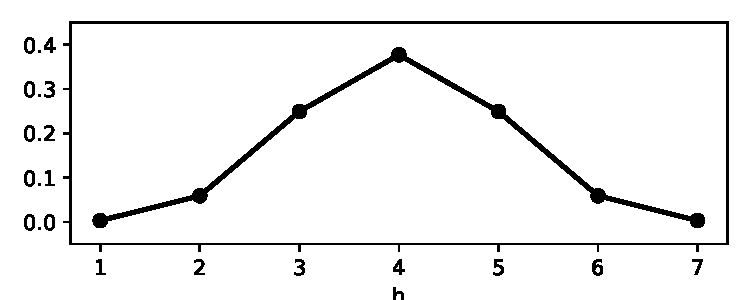
\includegraphics[width=0.9\columnwidth]{filter_coefficients.pdf}
    \qquad
\end{figure}

\begin{figure}[H]
    \centering
    \label{fig:response_curve}
    \caption{The expected response curve for an FIR low-pass filter built with the coefficients in Table \ref{tab:coeff}. The highest gain is below the cut-off frequency, while all frequencies above are attenuated. }
    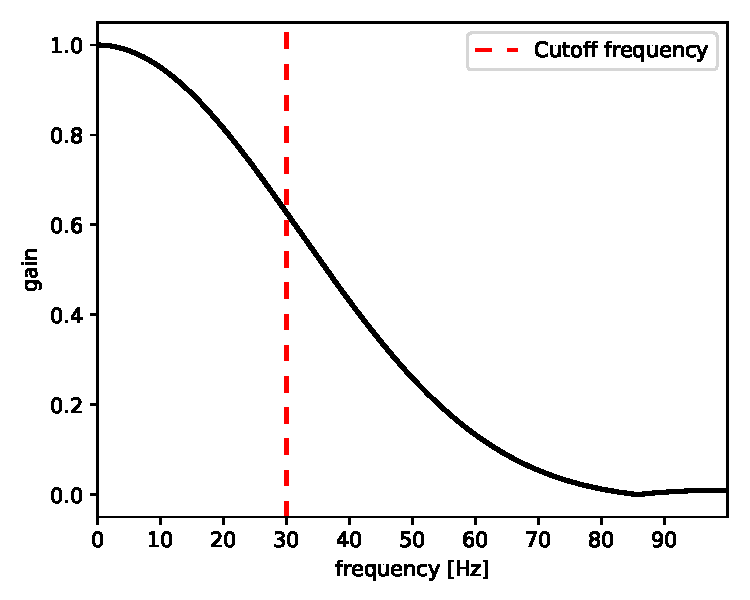
\includegraphics[width=1\columnwidth]{filter_response.pdf}
    \qquad
\end{figure}




\subsection{Symmetric coefficients}
\label{ssec:symmetric_coefficients}

Playing around with the coefficient computation, we noticed that the coefficients for high and low-pass filters are symmetric, i.e. the first coefficient is equivalent to the last one, the second to the second-last one and so on, in pairs. 
We use the fact that h is symmetric to do some fine optimization on the design. Explicitly, for 7-taps it means $h_0=h_6$ , $h_1=h_5$, $h_2=h_4$; $h_3$ remains unpaired. Therefore, the convolution of Eq. \ref{eq:7fir} can be rewritten as:
\begin{equation}
\begin{split}
    Y[n] = \; & h_0 (X_0+X_6) + h_1(X_1+X_5) + \\ 
           & + h_2(X_2+X_4) + h_3 \cdot X_3
\end{split}
\label{eq:7fir_optimized}
\end{equation}

The number of calculations to be implemented is only slightly reduced: the multiplications are substantially replaced by the sums, so one can hastily conclude that there is no advantage in doing so. However, this choice can be effective in terms of performance, as the 'trick' almost halves the number of multiplications to be performed. In FPGAs, the multiplications are way more complex than sums, so we can look after a performance gain. Since we are working with a filter of only 7 taps, this advantage is not as effective as it would be if we used a higher order filter. Indeed, for an odd number of taps:

\[ m^* = \textrm{multiplications to perform} = \frac{\textrm{taps}_{(odd)} + 1}{2} \sim \frac{\textrm{taps}}{2}\]





\section{Implementation of a FIR filter in VHDL}
\label{sec:implementation}

Now that all cards are on the table, we have to discuss the implementation on FPGAs.

As a design choice, we process the signal samples as 8-bit signed integers. This choice is forced by the fact that our UART module exchanges only 8-bit values for each transmission (duplex RS-232 standard). All the values are implemented in VHDL as signals, or vectors of signals when required. These conditions put boundaries on the input signal: samples must be provided as integer values in range $[-127, 128]$. Since the data is fed by a computer, we can account for this condition on the client side.

In VHDL, $X[n]$ is a vector of 7 signals, in which we store simultaneously the last 7 values of the input. Every time a new sample is fed to the FIR filter, the whole vector will shift so that the oldest sample is discarded, and the newest one will be placed as first element. The coefficients values are placed in another vector $h_k = h(k)$. These coefficients are static, unless explicitly changed. Therefore, every new incoming sample $X[j]$, the filter will multiply the stored inputs $X[i]$ to the associated coefficient $h_i$ and sum the multiplied values, the result of which will be eventually stored in $Y[j]$. Recall that $Y$ is just a single value passed directly to the UART interface, which sends the value to the computer client.

Although the coefficients are float values, as shown in §\ref{sec:firs}, we want to avoid floating point calculations. The main reason is that float operations in FPGAs are much more complex than integer operations; furthermore they would require a specific library. In order to overcome this issue, we proceed in the typical fashion of scaling the values and rounding them up, providing the right amount of significant digits. We chose to multiply the float coefficient by a power of two, and then we round the value to be a signed integer. The error committed on the rounding operation is negligible, as we will see in the results. To provide an example, if the coefficient was $h_i = 0.2453$:
\[0.2453 \cdot 2^8 = 62.7968 \simeq 63\]

The coefficients of Table \ref{tab:coeff} are rewritten, scaled and rounded, in Table \ref{tab:coeff_rounded}. We also show the hexadecimal 8-bit signed representation because numbers in VHDL code must be specified in this format.

\begin{table}[H]
    \renewcommand{\arraystretch}{1.2}
    \centering
    \caption{The FIR coefficients used as default filter specifications. The float values have been scaled by a factor of $2^8$, then rounded to the closest integer. We assume that the coefficients are symmetric, so we show only the first 4 values (out of 7 coefficients).}
    \label{tab:coeff_rounded}
    \scalebox{1.1}{
\begin{tabular}{ccc}
\hline
float      & rounded integers & hex   \\ \hline
0.00329661 & 1                & X"01" \\
0.05897323 & 15               & X"0f" \\
0.24920989 & 64               & X"40" \\
0.37704053 & 97               & X"61" \\ \hline
\end{tabular}
}
\end{table}

Since the convolution of the signal is linear, scaling the coefficients implies that also the output value $Y[j]$ is being scaled:
\[ Y^*[j] = 2^8 \cdot \sum_{i=0}^{6} h_i \cdot X[n-i] \]
\[ Y[j] = \frac{1}{2^8} Y^*[j] = \sum_{i=0}^{6} h_i \cdot X[n-i] \]
To get the unscaled output $Y[j]$, we simply have to shift back the output signal $Y^8[j]$ of 8-bits. This is why we scaled by a power of two: scaling back the output can be easily done on the FPGA with a costless signal crop.



\begin{table*}[hbp]
    \renewcommand{\arraystretch}{1.2}
    \centering
    \caption{The processes which manage the pipeline of Eq. \ref{eq:7fir_optimized} convolution. }
    \label{tab:pipeline}
\begin{tabular}{lllc}
\hline
\multicolumn{1}{c}{process} & \multicolumn{1}{c}{operation} & \multicolumn{1}{c}{target VHDL object} & \multicolumn{1}{c}{bits required} \\ \hline
\texttt{pipeline} & insert the new sample and shift the others & \texttt{x is array (0 to 6) of signed(7 downto 0);} & 8 (input) \\
\texttt{sum0} & sum the samples matching to the same coefficients & \texttt{x0 is array (0 to 3) of signed(8 downto 0);} & 9 \\
\texttt{mults} & multiply elements of x0 for the coefficients h & \texttt{m is array (0 to 3) of signed(16 downto 0);} & 17 \\
\texttt{sum1} & sum multiplication results in pair & \texttt{s1 is array (0 to 1) of signed(17 downto 0);} & 18  \\
\texttt{sum2} & sum the final values  & \texttt{output is std\_logic\_vector(18 downto 0);} & 19 \\ \hline
\end{tabular}
\end{table*}




\vspace{\fill}
\subsection{Pipeline of operations}
\label{ssec:pipeline}


The convolution of Eq. \ref{eq:7fir_optimized} is pipelined in multiple VHDL processes:
\begin{itemize}

    %\setlength\itemsep{0.6em}  % custom spacing for this listing

    \item \emph{Input pipeline} - The samples are progressively stored in $X[n]$. When a new sample is provided through the UART receiver, the old ones are shifted one place to the right and the last one is discarded.
    \newpage
\begin{lstlisting}[ basicstyle=\small, language=VHDL]
pipeline : process(clk) is
begin
  if active = '0' then
    x <= (others=> (others=>'0'));
  elsif rising_edge(clk) then
    if Din_valid = '1' then
      x <= signed(Din) & x(0 to order-1);
    end if;
  end if;
end process;
\end{lstlisting}
    
    
    \item \emph{Initial addition} - The samples that are going to be multiplied by the same coefficient are summed. In the case of the isolated $X[3]$ we would use a flip-flop to hold the value as the first 3 additions are performed. This is necessary to keep synchronized all the operations. 
    
    In practice, we store the first 3 additions in a vector of signals, and at the same time we redirect the isolated $X[3]$ as the last element of the vector.
    
\begin{lstlisting}[ basicstyle=\small, language=VHDL]
sum0 : process(clk) is
begin        
  if rising_edge(clk) then
    if Din_valid = '1' then
      for i in 0 to 2 loop
        x0(i) <= resize(x(i),9) + resize(x(6-i),9);
      end loop;
           
      x0(3) <= resize(x(3),9);
    end if;
  end if;
end process;
\end{lstlisting}
    
    
    \item \emph{Multiplications} - The vector coming from the first addition is multiplied (element-wise) by the coefficients.
    
\begin{lstlisting}[ basicstyle=\small, language=VHDL]
mults : process(clk) is
begin
  if rising_edge(clk) then
    if Din_valid = '1' then
      for i in 0 to 3 loop
        m(i) <= x0(i) * signed(coeffs(i));
      end loop;
    end if;         
  end if;
end process;
\end{lstlisting}


    \item \emph{Next additions} - The products are added all together. This requires two subsequent parallel processes.

\begin{lstlisting}[ basicstyle=\small, language=VHDL]
sum1 : process(clk) is
begin
  if rising_edge(clk) then
    if Din_valid = '1' then
      for i in 0 to 1 loop
        s1(i) <= resize(m(2*i),18) + 
                 resize(m(2*i+1),18);
      end loop;
    end if;    
  end if;
end process;

sum2 : process(clk) is
begin
  if rising_edge(clk) then
    if Din_valid = '1' then
      output <= std_logic_vector( 
                 resize(s1(0),19) + 
                 resize(s1(1),19) );
    end if;
  end if;
end process;
\end{lstlisting}


    \item \emph{Output} - The output is suitably shifted.

\begin{lstlisting}[ basicstyle=\small, language=VHDL]
-- in final entity
vout <= output(15 downto 8);
\end{lstlisting}

\end{itemize}

Since we are implementing the values as VHDL signals, we have to manually manage the size of such entities. The rules for binary operations are simple:
\begin{itemize}
    \item multiplication between two numbers, one of $a$ bits and another of $b$ bits, is a number of $a+b$ bits;
    \item addition of two numbers, one of $a$ bits and another of $b$ bits, is a number of $max(a,b)+1$ bits.
\end{itemize}
According to these rules, Table \ref{tab:pipeline} shows a recap of the pipeline operations and the suitable bit size of the VHDL entities.


\begin{figure}[H]
    \centering
    \caption{A schematic representation of the pipelined operations. The processes are described in §\ref{ssec:pipeline} and further summarized in Table \ref{tab:pipeline}.}
    \label{fig:scheme_symmetric}
    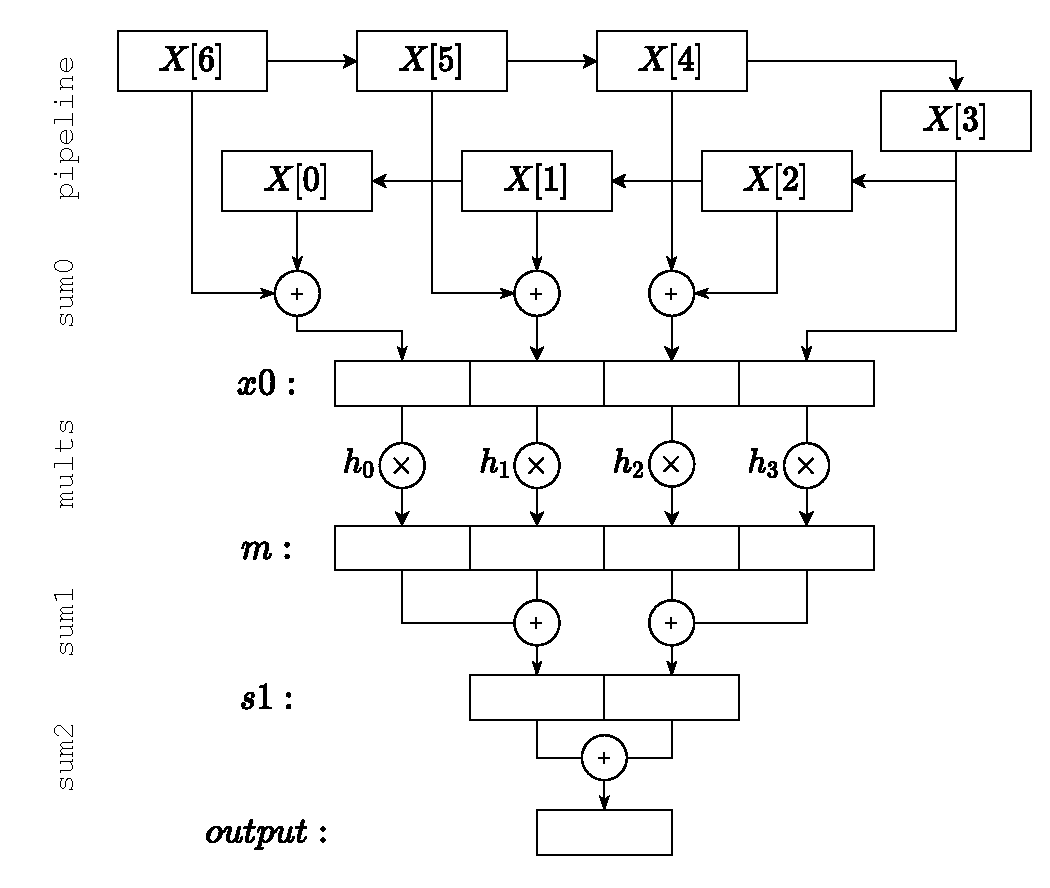
\includegraphics[width=1\columnwidth]{7fir_draw.pdf}%}
    \qquad
\end{figure}



\newpage
\subsection{UART module}
\label{ssec:uart}

The UART is a device which allows duplex data exchange between two clients. In our project, this protocol is used to exchange 8-bit signed values from/to the FPGA. To set up the UART correctly, the clients (computer and FPGA) must agree on how quickly the data is transferred - this speed is called baud-rate, and our implementation is working at baud-rate 115200.

Following the RS-232 standard, the 'idle' state (in which the receiver is waiting for data) is HIGH (1). Each transmission begins with a LOW (0) status and ends with a HIGH after the 8 bits have been transmitted.

\begin{figure}[H]
    \centering
    \label{fig:uart_std_protocol}
    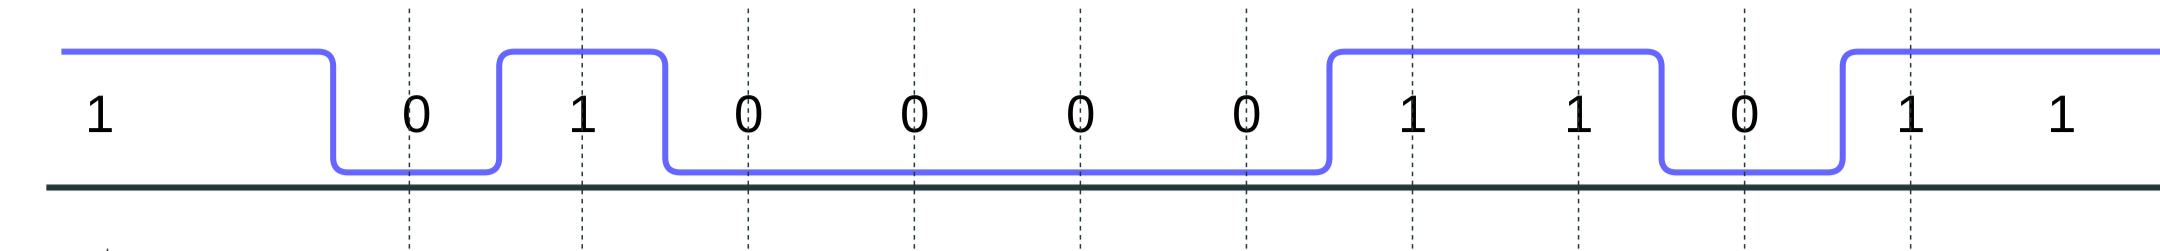
\includegraphics[width=0.94\columnwidth]{uart_protocol.png}
    \qquad
\end{figure}

The UART entities (RX and TX) can be included externally with the following code.

\begin{lstlisting}[ basicstyle=\small, language=VHDL]
component uart_tx_module is
  port( clk, data_valid : in std_logic;
        data_to_send : in
          std_logic_vector(7 downto 0);
        busy, uart_tx : out std_logic );
end component;
    
component uart_rx_module is
  port( clk, uart_rx  : in std_logic;
        valid : out std_logic;
        received_data : out 
          std_logic_vector(7 downto 0));
end component;
\end{lstlisting}


\subsection{FIR filter entity for FPGA}
\label{ssec:entity}

Finally, all the previous entities are joined to create a functional FIR filter. In the FPGA, the receiver module obtains data from the USB interface. The data is sent to the FIR Filter, where it is processed and then sent to the transmitter module. The other side of the USB interface is managed through Python scripts.

\begin{figure}[H]
    \centering
    %\subfigure[]{
    \label{fig:fpga_scheme}
    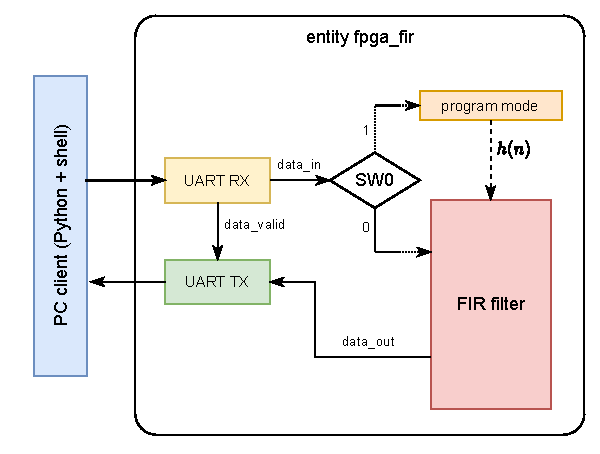
\includegraphics[width=1.0\columnwidth]{fir_entity_draw.pdf}%}
    \qquad
\end{figure}



\section{Filter simulation on Vivado}
\label{sec:simulations}

Before testing the filter on the real FPGA, we did some tests on Vivado simulations. We wrote a test-bench which takes the signal samples from a txt file and feeds them to the FIR filter. 

\begin{figure}[H]
    \centering
    \label{fig:simulator}
    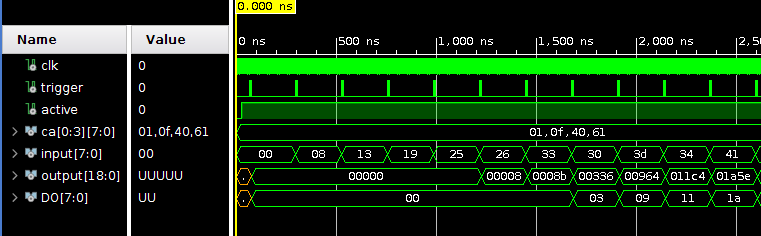
\includegraphics[width=1\columnwidth]{vivado_simulation.png}
    \qquad
\end{figure}

The simulation shows that the latency in the output update is of 5 sampling cycles. This latency agrees with our expectations, since the pipeline process breaks the operations in 5 processes. This design can be further improved by making the computation processes sensible to the clock, instead of the \texttt{data\_valid} impulse provided by the UART receiver module. Since the UART works at a sampling frequency 2-magnitudes smaller with respect to the 100MHz clock of the FPGA, we are sure that the output could be refreshed in less than a sampling cycle.

\begin{figure}[H]
    \centering
    \label{fig:simulated_waveform}
    \caption{Results of a Vivado simulation of the FIR filter. In this simulation, a noisy waveform is fed to the FIR filter and output is stored in memory. The input signal is the noisy wave plotted in grey; it has been obtained summing a carrier 5Hz sine wave to higher frequencies noise. The Vivado simulation output is the yellow curve. One can also notice that the Vivado output perfectly overlaps the Python FIR (blue curve) which has been obtained simulating in Python a FIR filter of equivalent specifications as our FPGA FIR filter. This further assures us of the correctness of the implemented convolution.}
    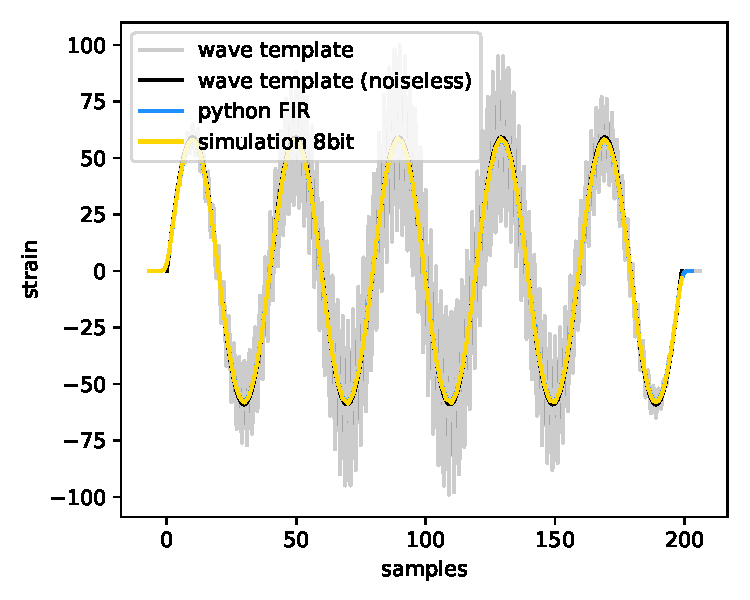
\includegraphics[width=1\columnwidth]{simulated_waveforms.pdf}
    \qquad
\end{figure}

\section{Run-time coefficient re-programming}
\label{sec:real_time}

We have added a special functionality to our FIR filter implementation: a \emph{programming mode} that allows us to change run-time the FIR coefficients. This is advantageous, because it allows to change the filter specifications without running again the implementation on Vivado, which is notoriously a time-consuming step. 

Hands on, the coefficients are re-programmed through this steps:
\begin{itemize}
    \item enable \texttt{programming mode} - Close SW0 on the FPGA board. The status LED becomes red.
    \begin{figure}[H]
    \centering
    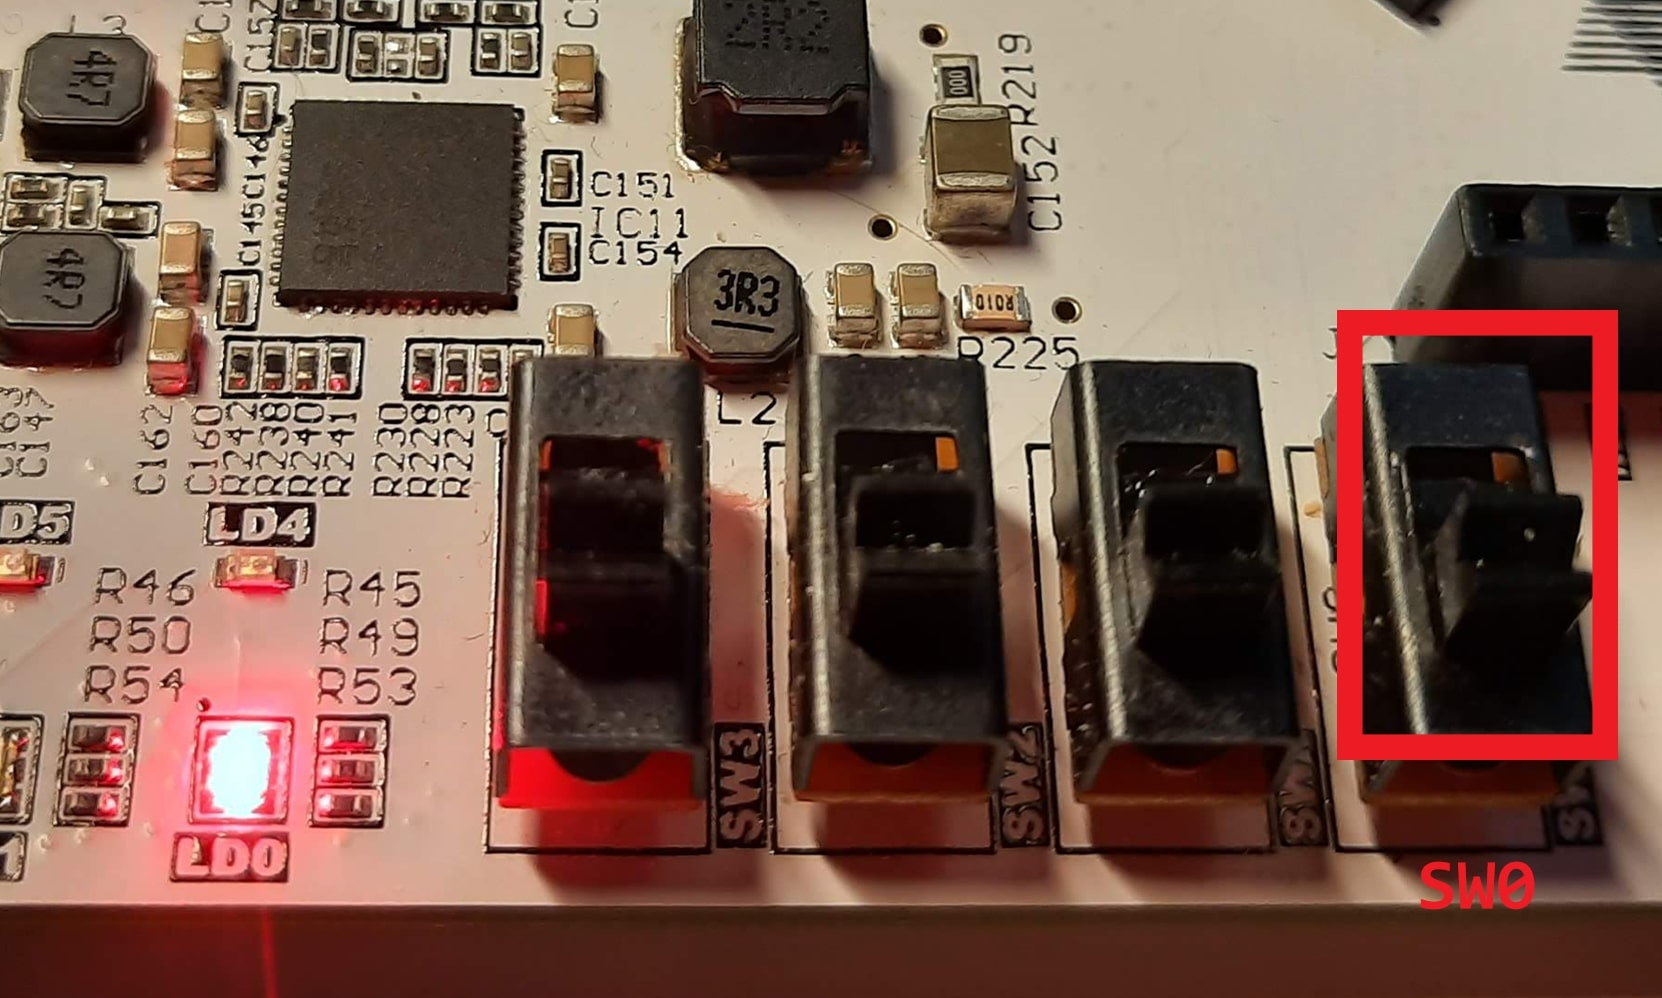
\includegraphics[width=0.7\columnwidth]{demo_programming.jpg}
    \end{figure}

    \item send the new coefficients - The board is now ready to receive the new coefficients. Use the Python scripts to send them. When all coefficients have been received, the status LED turns purple.
    \begin{figure}[H]
    \centering
    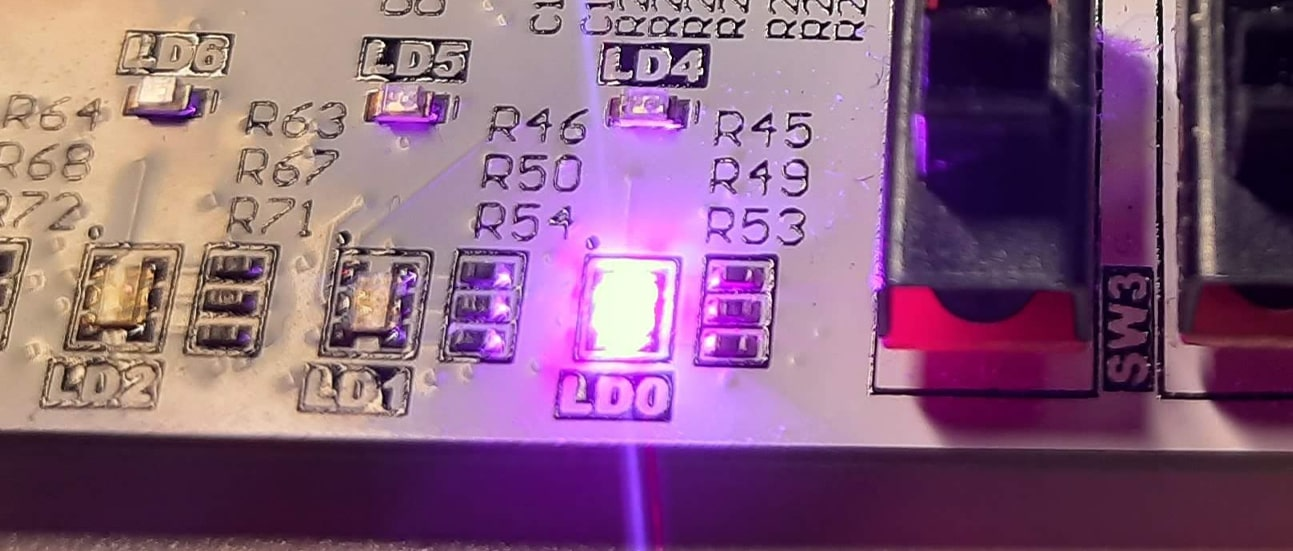
\includegraphics[width=0.7\columnwidth]{demo_acquired.jpg}
    \end{figure}
    
    \item go back to \texttt{filter mode} - Open SW0 on the FPGA board. The status LED turns green. The board is ready to receive the values to process with the FIR filter.
    \begin{figure}[H]
    \centering
    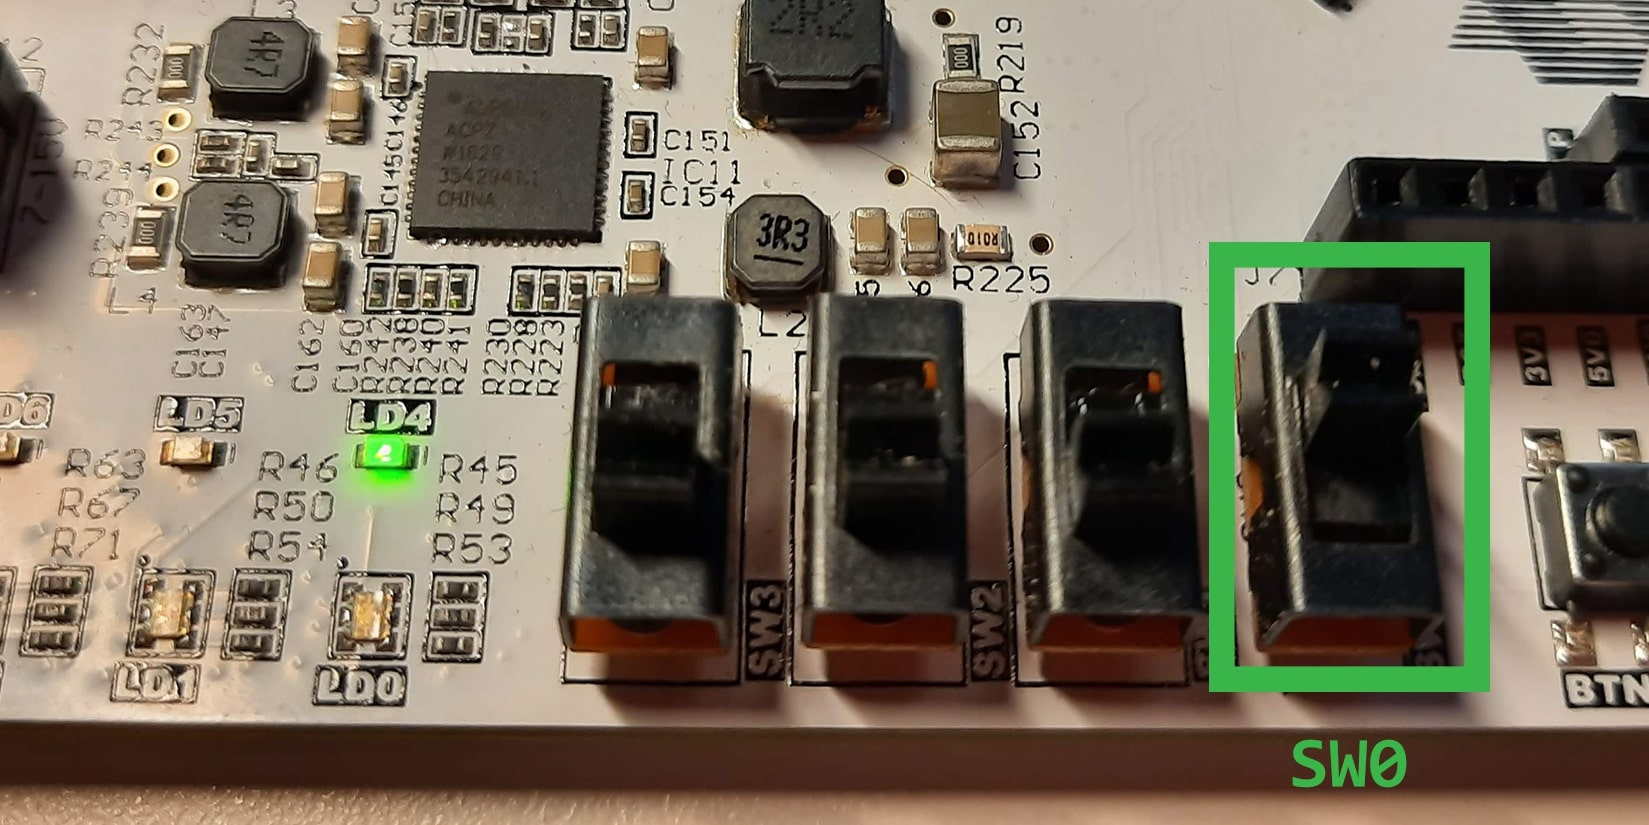
\includegraphics[width=0.7\columnwidth]{demo_filter.jpg}
    \end{figure}
\end{itemize}



\section{Front-end interface}
\label{sec:frontend}

To manage the I/O on the computer side, we created some Python scripts. The script \texttt{send\_data\_fpga.py} is meant to fed the FPGA an input waveform and retrieve the filtered output. The waveforms must be provided through a txt file with 8-bits signed integer values, one for each row. Instead, when the FPGA is in programming mode (red LED), we can set the coefficients using the script \texttt{write\_coefficients.py}. The coefficients are specified as arguments in the shell (use the \texttt{-c} flag). The following lines of code show a brief example on how those commands should be called on a bash shell:
\begin{lstlisting}[language=bash]
./tools/write_coefficients.py -c 0 8 32 48
./tools/send_data_fpga.py -i INPUT.txt -o OUTPUT.txt
\end{lstlisting}

To make even easier to program the FPGA, we created a tlc script for Vivado, which automatically setups the FPGA and loads an optimal bitstream from the \texttt{/bit} folder. Run it with
\begin{lstlisting}[language=bash]
./tools/program_fpga.sh
\end{lstlisting}

In the project folder there are also 3 Jupyter notebooks, which we used to perform the analysis and get the results shown in §\ref{sec:results}. 






\subsection{Demo}
\label{ssec:switching_demo}

\begin{figure}[H]
    \centering
    \caption{}
    \label{fig:demo_switch_general}
    \subfigure[Low-pass configuration. $h_k =  1, 8, 32, 48$. ]{
    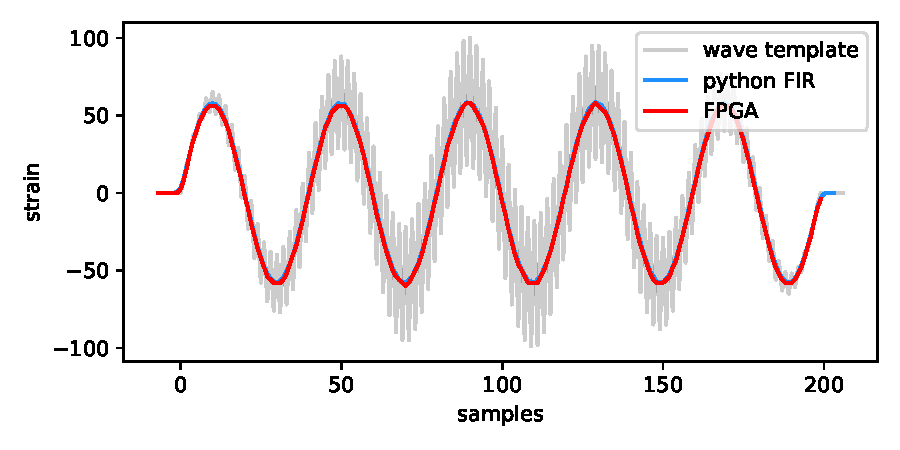
\includegraphics[width=1.0\columnwidth]{demo_lowpass.pdf}}
    \label{fig:demo_switch_lowpass}
    
    
    \subfigure[High-pass configuration. $h_k = 1, -6, -25, 89$. ]{
    
    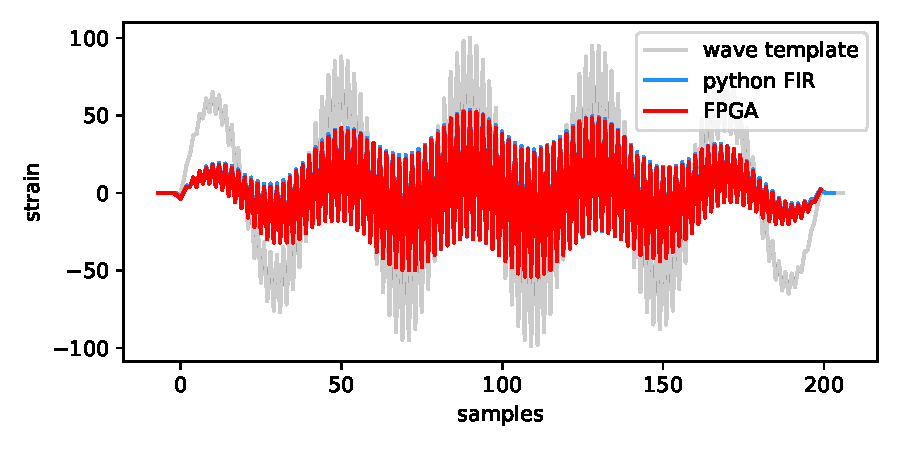
\includegraphics[width=1.0\columnwidth]{demo_highpass.pdf}}
    \label{fig:demo_switch_highpass}
    \qquad
\end{figure}

Let us quickly show the results of a demo which we arranged on a Jupyter notebook (\texttt{7fir\_demo\_switch.ipynb}). The target of this demo is to prove the effectiveness of the re-programming feature in our implementation. In order to do so, we first setup the FPGA to be a low-pass filter with cut-off frequency of 30Hz. We feed to the FPGA a sample noisy waveform and retrieve the filtered waveform [Figure \ref{fig:demo_switch_lowpass}a]. Then, we set new coefficients in the FPGA: this time to make the filter work as an high-pass filter with cut-off frequency of 30Hz. Finally, we feed the previous input noisy waveform and retrieve the output [Figure \ref{fig:demo_switch_highpass}b]. Comparing the results, we can clearly see that the filter works as expected in both cases. The advantage of our implementation is that we can easily switch the coefficients run-time, without writing again the bitstream.




\begin{figure}[hbt]
    \centering
    \caption{Simulated noisy waveforms, sampled at 200 Hz.}
    \label{fig:sample_general}
    
    \subfigure[5 Hz sine wave + 100 Hz sine noise.]{
    \label{fig:sample_sine}
    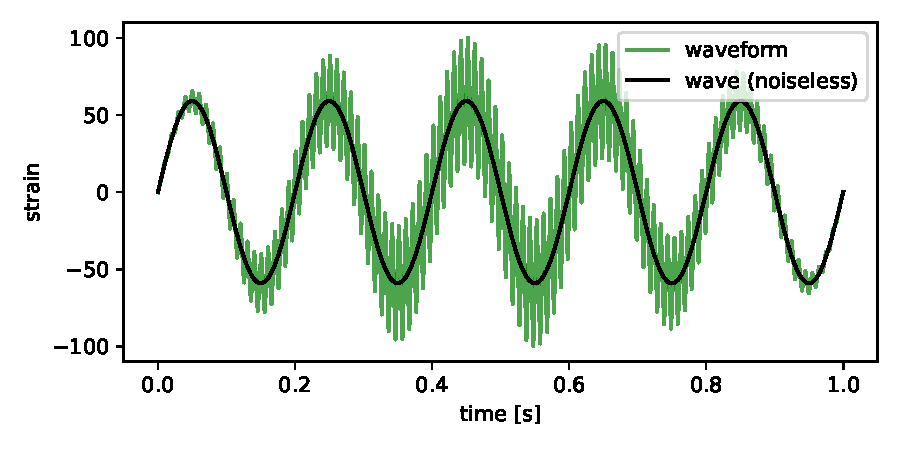
\includegraphics[width=1.0\columnwidth]{wwsample_sine.pdf}}
    
    \subfigure[Two gaussian pulses with 80Hz noise.]{
    \label{fig:sample_gaussian}
    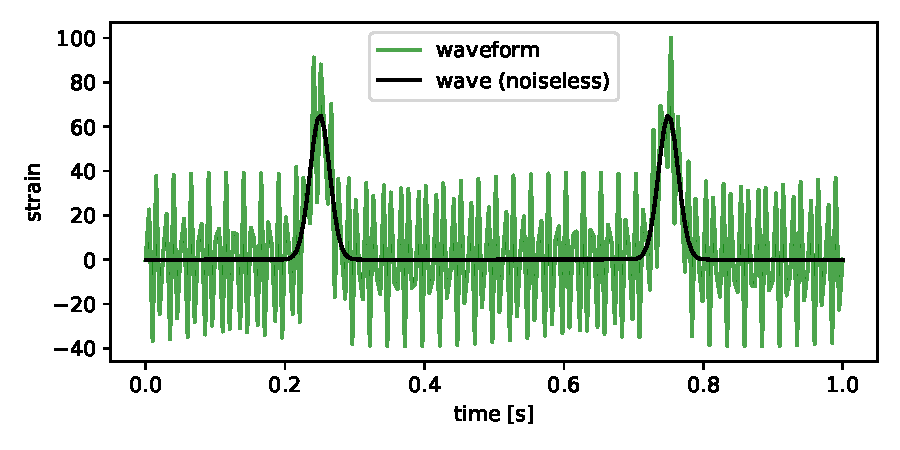
\includegraphics[width=1.0\columnwidth]{wwsample_gaussian.pdf}}
    
    \subfigure[An electrocardiogram taken from the Scipy package, with random gaussian noise.]{
    \label{fig:sample_ecg}
    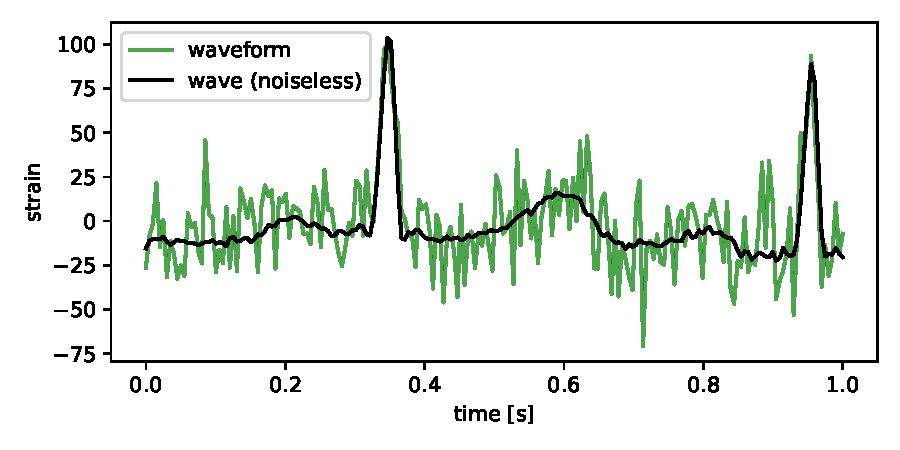
\includegraphics[width=1.0\columnwidth]{wwsample_ecg.pdf}}
    \qquad
\end{figure}


\begin{figure}[hbt]
    \centering
    \caption{ The noisy waveforms of Figure \ref{fig:sample_general} processed by the FPGA. The FPGA output matches with the python FIR filter which uses the same coefficients as the FPGA.}
    \label{fig:real_general}
    
    \subfigure{
    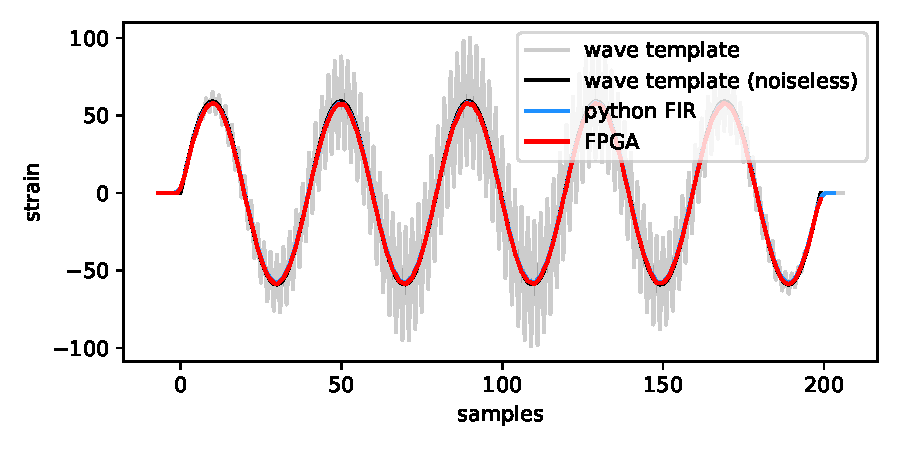
\includegraphics[width=1.0\columnwidth]{wwreal_sine.pdf}}
    
    \subfigure{
    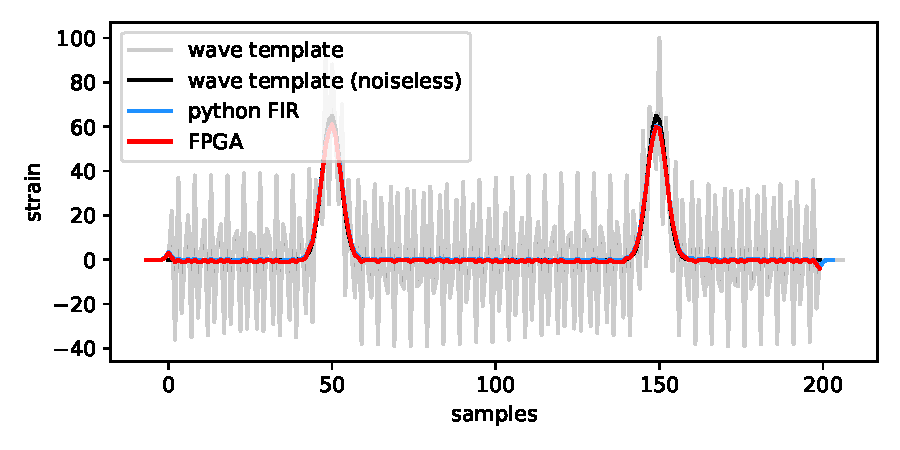
\includegraphics[width=1.0\columnwidth]{wwreal_gaussian.pdf}}
    
    \subfigure{
    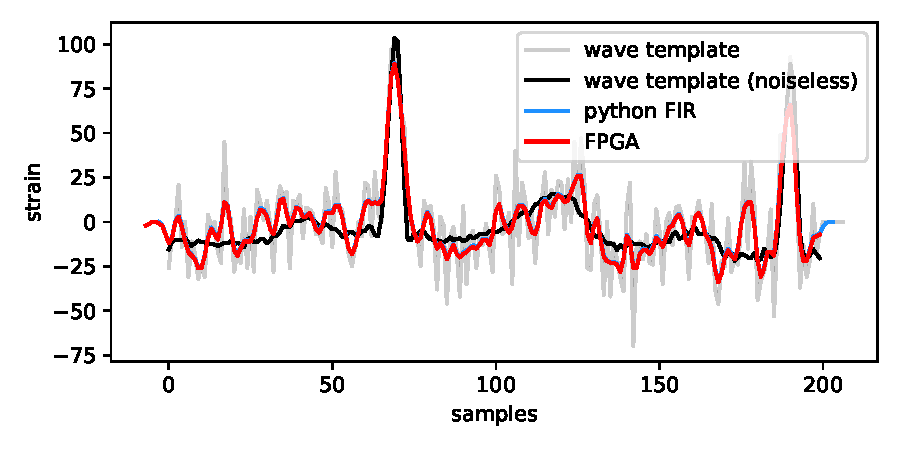
\includegraphics[width=1.0\columnwidth]{wwreal_ecg.pdf}}
    \qquad
\end{figure}



\section{Results and discussion}
\label{sec:results}

% Bahador text here

In this last section we will discuss some results of the implemented FIR filter, applying it to different waveform samples.

First, we simulate different carrier waveforms and add high frequency noise to them. We will consider three kinds of carrier waveforms, which are a 5 Hz sine wave, two gaussian pulses and electrocardiogram wave. In Figures \ref{fig:sample_general} we show the corresponding trend of each carrier waveform (black line), as well as the final noised waveform (green line).

At this stage we have some artificially generated noised waveforms. The noised waveforms are given as an input to our FPGA FIR filter and the output is memorized by the computer client through the Python scripts introduced in §\ref{sec:frontend}. To provide a better comparison, we also performed a low-pass filtering through Scipy library. The Python low-pass filter is internally implemented as an FIR filter, which has the same specifications as our FIR FPGA. Therefore we expect that FPGA FIR output matches with the theoretically equivalent Python FIR filtering.




% captions
%We start with sine noised waveform
%


%We plotted 4 different graphs. The original waveform, the Noised Waveform, the result of Python Fir and finally the result of our FPGA.

%[results for Gaussian and ECG]%, if some cool points about these graphs were noticed, we should mention it otherwise the description is generally the same as the sine noise waveform.


As we can see in Figures \ref{fig:real_general}, FPGA filtering works properly and matches the Python FIR filter. More importantly, the filtered waveform generally matches with the noiseless waveform sample. The only exception is the ECG waveform, since it has been soiled with gaussian random noise, which is hard to filter out using frequency thresholds. These results show that our FPGA FIR filter is capable of removing all the high-frequency noise and seems to be a successful low-pass filter.


\subsection{A guitar experiment}
\label{ssec:demo_guitar}

As a final demonstration, we wish to probe the performance of our FIR filter on a real-world application. Our experiment involves the world of electric guitars and musical signal processing. We try to simulate an electric guitar \emph{pickup selector} with our FIR filter. The pickup selector is a physical switch on electric guitar which allows the guitar player to choose between different pickups or a combination of them.

\begin{figure}[H]
    \centering
    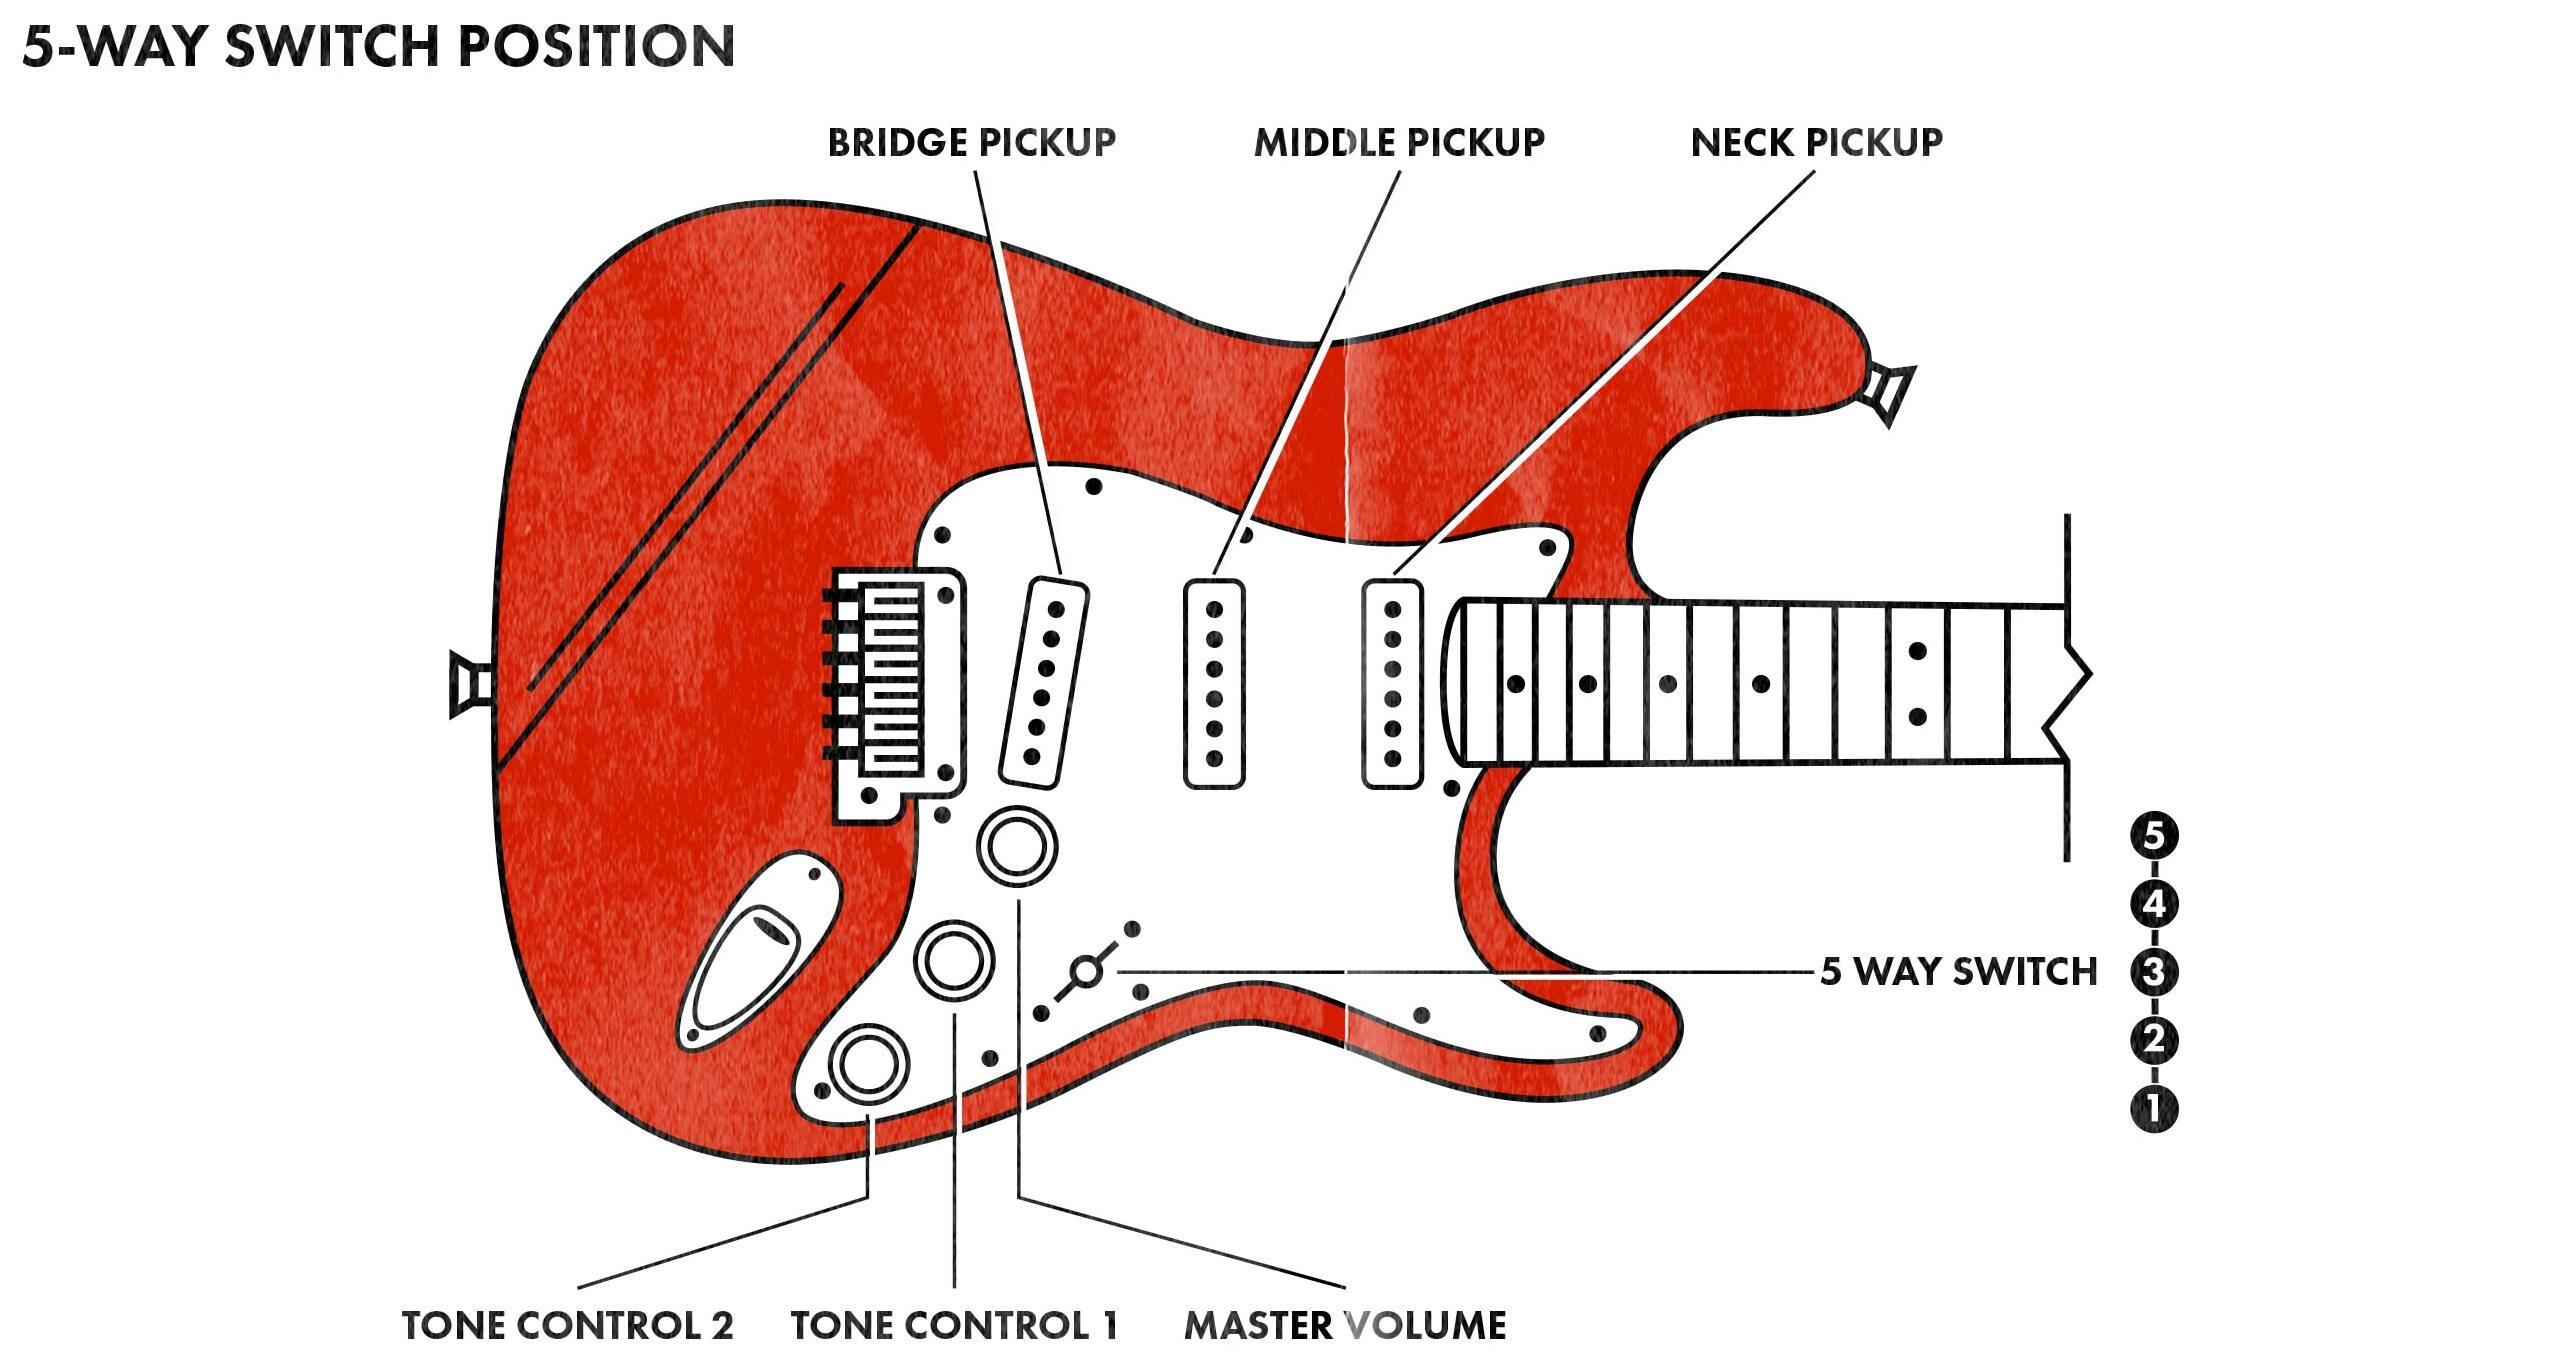
\includegraphics[width=0.9\columnwidth]{guitar_selector.jpg}
    % put reference to original pic!
\end{figure}

\emph{What makes pickups different?} “The bridge pickup produces a brighter tone than the neck pickup which sounds warmer and more mellow. Often, the bridge pickup is used for lead guitar and heavier styles of music with more gain such as rock and metal, whilst the neck pickup is used for rhythm guitar and cleaner tones”\cite{pickup_guitar}.

To put it in a more physical perspective, each musical instrument has its peculiar sound (timbre) which is given by a combination of frequencies. The sound of a violin, for instance, is differently distributed among frequencies with respect to a piano. The guitar pickups act on the frequencies distributions, so that the timbre of the guitar changes. 
A \emph{bridge pickup} spans higher frequencies, while the neck pickup spans lower frequencies. The pickup changes the balance among the two ranges, so that the sound of the guitar becomes, respectively, sharper or warmer.

In order to not get confused with musical expressions, we will refer to these concepts using another notation: we consider two modes for the pickup selector, the \emph{high-mode} and the \emph{low-mode}. The high-mode corresponds to a sharper sound (i.e. enhanced higher frequencies) and the low-mode to a deeper sound (i.e. enhanced lower frequencies). With a certain approximation, we can try to simulate this effects respectively with an high-pass and a low-pass filter.

Using an electronic guitar and a smart amplifier, we recorded a specific note, the E (open string) (dominant frequency 329Hz), one time with the pickup in low-mode and another in high-mode. Furthermore, we repeated the process using multiple amplifiers setting. Each amplifier configuration leads to a unique timbre: although the played note is still the same, the amplifier produces a different timbre. Recorded signals are finally gathered in a sound bank, distinguishing between timbres. In our demo code, we can select a specific timbre from the sound bank:
\texttt{ [Clean, Acoustic, Funk Wah, High Gain, Metallica] }.


For example, considering a “Clean” timbre, we plot a tiny slice of signal to see what’s going on.
\begin{figure}[H]
    \caption{}
    \centering
    \subfigure[High-mode: the signal is characterized by higher frequencies, so the timbre will be sharper.]{
    \label{fig:guitar_clean_high_raw}
    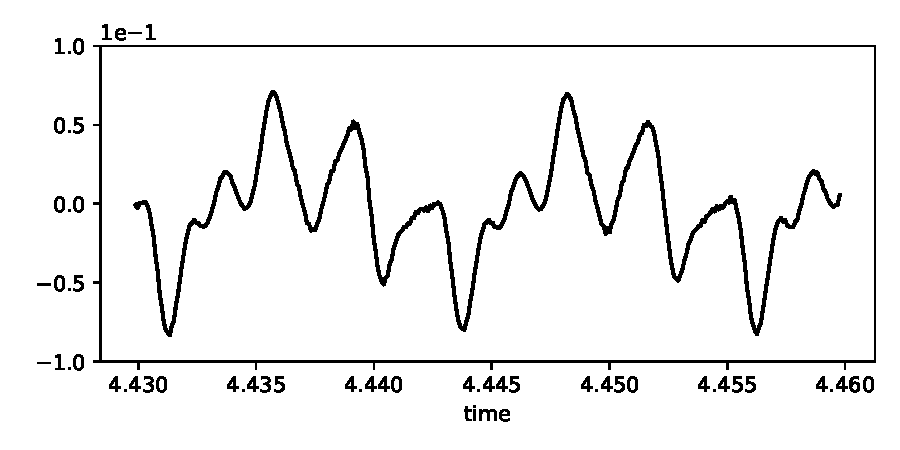
\includegraphics[width=1.0\columnwidth]{clean_high_raw.pdf}}
    
    \subfigure[Low-mode: higher frequencies are attenuated in favour of lower ones, so the timbre will be deeper, even if the carrier wave appears to be untouched.  ]{
    \label{fig:guitar_clean_low_raw}
    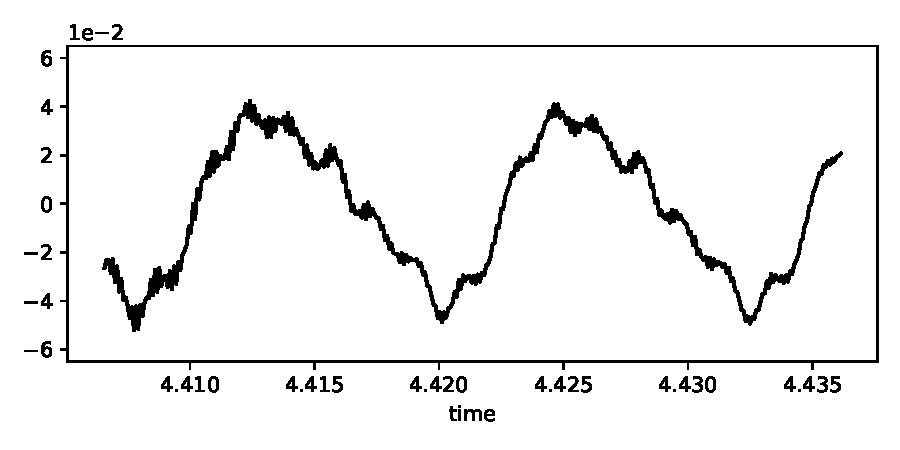
\includegraphics[width=1.0\columnwidth]{clean_low_raw.pdf}}
    \qquad
\end{figure}

Our goal is simply to simulate the low-mode signal starting from the recorded high-mode signal, using a FIR low-pass filter. Indeed, by filtering out the higher frequencies we expect the transformed signal to be more powerful on the lower frequencies band, miming the low-mode signal produced by guitar pickup selector. Eventually, we can compare the FIR output to the low-mode recorded sample. Since we have shown in §\ref{sec:simulations} that the FPGA FIR output always matches with the Python simulations, in order to optimize our analysis we will consider, from now on, only FIR Python simulations.

\begin{figure}[H]
    \centering
    \caption{Pickup simulation on the "Clean" sound bank sample. The plot shows that the simulated 45-taps low-pass filter is capable of achieving greater similarity wrt the real pickup.}
    \label{fig:clean_processed}
    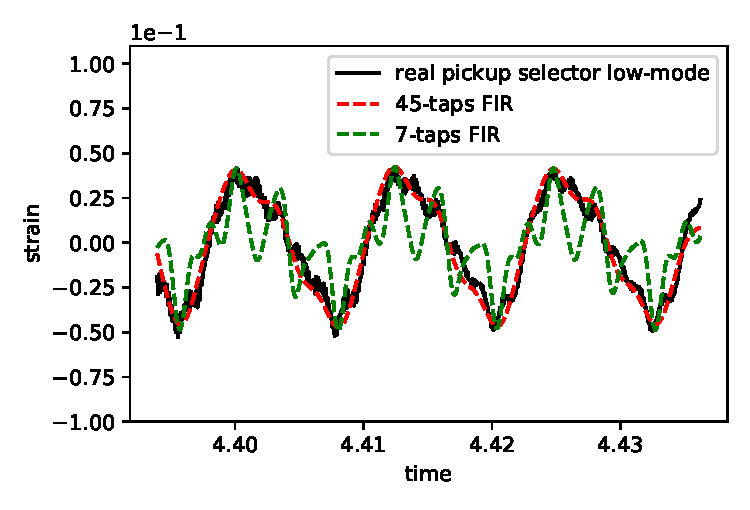
\includegraphics[width=1\columnwidth]{clean_processed.pdf}
\end{figure}

The results of this processing is shown in Figure \ref{fig:clean_processed}. One can observe that the low-mode signal simulated through a 7-taps FIR filter does not properly match the actual low-mode signal of the guitar pickup selector. However, if we increase the number of taps, for example to 45, we are able to achieve a greater degree of similarity: the FIR processed waveform resembles the waveform recorded using a real guitar pickup selector.


\begin{figure}[H]
    \centering
    \caption{Pickup simulation on the "Acoustic" sound bank sample.}
    \label{fig:other_processed}
    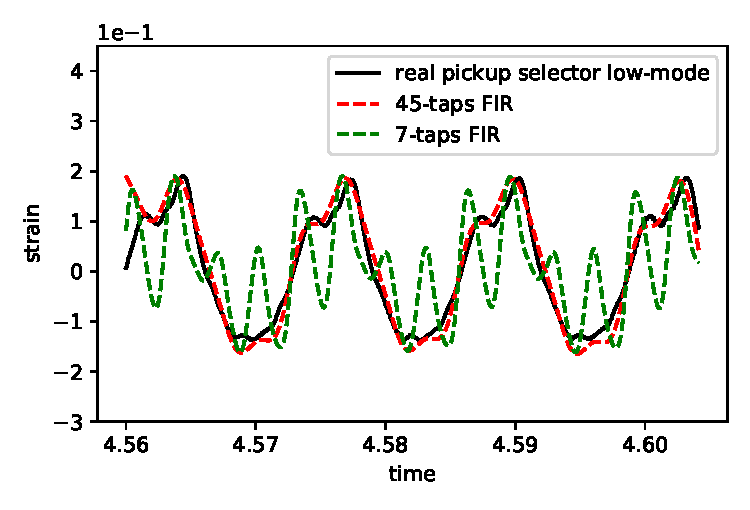
\includegraphics[width=1\columnwidth]{other_processed.pdf}
\end{figure}

Figure \ref{fig:other_processed} show the same filtering performed on other timbres from our sound bank. The outcome is a bit different for each sample, but the general trend remains unchanged.



Our results do not prove wrong the idea of simulating low-mode pickup selectors with low-pass filters. Instead, they point out that these sound-tuning tasks require higher precision on the convolutions. Therefore, we would need an higher number of taps.


\section{Conclusions}
\label{sec:conclusions}

The implemented FIR filter, as shown by results, is capable of working both as a low-pass and high-pass filter. The simulations agree with the actual behaviour on FPGA boards, proving the correctness and efficiency of the design. To further improve the effect on real sound applications we suggest to increase the number of taps. As a side effect, such change would make more effective the design optimization we introduced due to the symmetric coefficients, reducing the amount of multiplications to perform. Finally, the feature which allows to change run-time the coefficients is a great advantage when it comes to test the FIR FPGA on various settings.

% coda
\vspace{\fill}
\par\par\noindent\rule{\columnwidth}{0.4pt}
\section*{Additional resources}
\centering{ The code of this project is available in a \\ GitHub repository.}
\begin{table}[H]
    \centering
    \renewcommand{\arraystretch}{1.8}
    \scalebox{1.2}{
\begin{tabular}{cl}
\hline
{\large\faGithub} & \href{https://github.com/baronefr/mapd_7taps_fir}{baronefr/mapd\_7taps\_fir } \\ \hline
\end{tabular}
}
\end{table}
\bibliographystyle{IEEEtran}
\bibliography{IEEEabrv,refs}

\end{document}